% article example for classicthesis.sty
\documentclass[10pt,a4paper]{article} % KOMA-Script article scrartcl
\usepackage{import}
\usepackage{xifthen}
\usepackage{pdfpages}
\usepackage{transparent}
\newcommand{\incfig}[1]{%
    \def\svgwidth{\columnwidth}
    \import{./figures/}{#1.pdf_tex}
}
\usepackage{lipsum}     %lorem ipsum text
\usepackage{titlesec}   %Section settings
\usepackage{titling}    %Title settings
\usepackage[margin=10em]{geometry}  %Adjusting margins
\usepackage{setspace}
\usepackage{listings}
\usepackage{amsmath}    %Display equations options
\usepackage{amssymb}    %More symbols
\usepackage{xcolor}     %Color settings
\usepackage{pagecolor}
\usepackage{mdframed}
\usepackage[spanish]{babel}
\usepackage[utf8]{inputenc}
\usepackage{longtable}
\usepackage{multicol}
\usepackage{graphicx}
\graphicspath{ {./Images/} }
\setlength{\columnsep}{1cm}

% ====| color de la pagina y del fondo |==== %
\pagecolor{black}
\color{white}



\begin{document}
    %========================{TITLE}====================%
    \title{{  Apuntes tema 07 Rodrigo Castillo Camargo  }}
    \author{{Rodrigo Castillo}}
    \date{\today}

    \maketitle


     % ====| Loguito |==== %
    
\includegraphics[width=0.1\linewidth]{negro_cara.png}
    %=======================NOTES GOES HERE===================%

    \section{cuando la varianza muestral generalizada es 0}
        la varianza generalizada es cero \color{red} cuando y solo cuando
        \color{white}  al menos un vector desviacon yace en el hiperplano
        formado por todas las combinaciones lineales , osea,  cuando las
        clumnas de la matriz de deviaciones es linealmente depengientes
        \begin{figure}[h!]
            \centering
            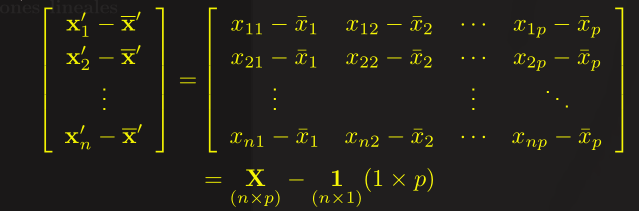
\includegraphics[width=0.8\linewidth]{matrizdesviaciones.png}
            \caption{matriz de desviaciones}
            \label{matriz desviaciones}
        \end{figure}

        que sucede cuando se crea una variable que es combinacion lineal de las
        otras?
        \begin{itemize}
            \item {una matriz de covarianza es \color{red} singular
                \color{white}  cuando los datos son puntajes de pruebas y el
                investigador ha incluido variables como sumas de las de mas}
            \item {esta es una \color{red} mala práctica \color{white} }
        \end{itemize}

        que pasa cuando se crea una variable combinacion lineal de las otras?

        \begin{enumerate}
            \item { $ Sa = 0  $  a es un vector propio}
            \item {$ a'(x_j  \hat{x} =0 paratodo j  $   la combinacion de los
                datos corregidos por la media usando $ a  $ es 0}
        \end{enumerate}


    \section{varianza generalizada determinada por $ R  $ }
        \begin{itemize}
            \item {la varianza de la muestra generalizada se ve afectada}
            \item {por ejemplo suponga que $ s_{ii}  $  es grande o muy
                pequeño, entonces geométricamente el vector de desviacion
                correspondiente $ d_i ? (y_i - \hat{x_i}  )  $  será muy largo o
                muy corto y \color{red} afectara el volumen \color{white} }
            \item {en conecuencia a veces es util escalar todos los vectores de
                desviacion para que tengan la misma longitud}
        \end{itemize}

        para escalar un vector  $  x_{kj}  $  \color{red} hacememos $
        \frac{x_{kj}- \hat{x_k}}{\sqrt{S_{kk}} }   $  \color{white}

        por lo ranto tenemos que $ R  $ es grande cuando todos los $ r_{ik}
        $ son casi 0 y es pequeño cuando uno o mas de los $ r_{ik}  $  son casi
        1 o -1

    \section{Varianza Generalizada}
       varianza generalizada ...
       \begin{equation}
           \color{red} varianza_{generalizada} = s_{11} + s_{22} + s_{33} + ...
           + s_{pp}
            \color{white}
        \end{equation}











    %=======================NOTES ENDS HERE===================%

    % bib stuff
    \nocite{*}
    \addtocontents{toc}{{}}
    \addcontentsline{toc}{section}{\refname}
    \bibliographystyle{plain}
    \bibliography{../Bibliography}
\end{document}
